%===========================================================
\documentclass[10pt]{article}
\usepackage[a4paper]{geometry}
\usepackage[T1]{fontenc}
\usepackage{CJKutf8}
\usepackage{graphicx}
\usepackage{alltt}
\usepackage{caption}
\usepackage{hyperref}
\captionsetup[figure]{labelformat=empty}
\captionsetup[table]{labelformat=empty}

\pagestyle{plain}
\thispagestyle{plain}
%===========================================================
%                          Title
%===========================================================
\title{HBF-701 Unofficial English Manual}
\author{Peter Senna Tschudin\footnote{I do not work for Omron. I just own one
HBF-701}\\ {\small peter.senna@gmail.com}}
\begin{document}
\maketitle
%===========================================================
%                          Title
%===========================================================
\begin{center}
\vspace{15pt}
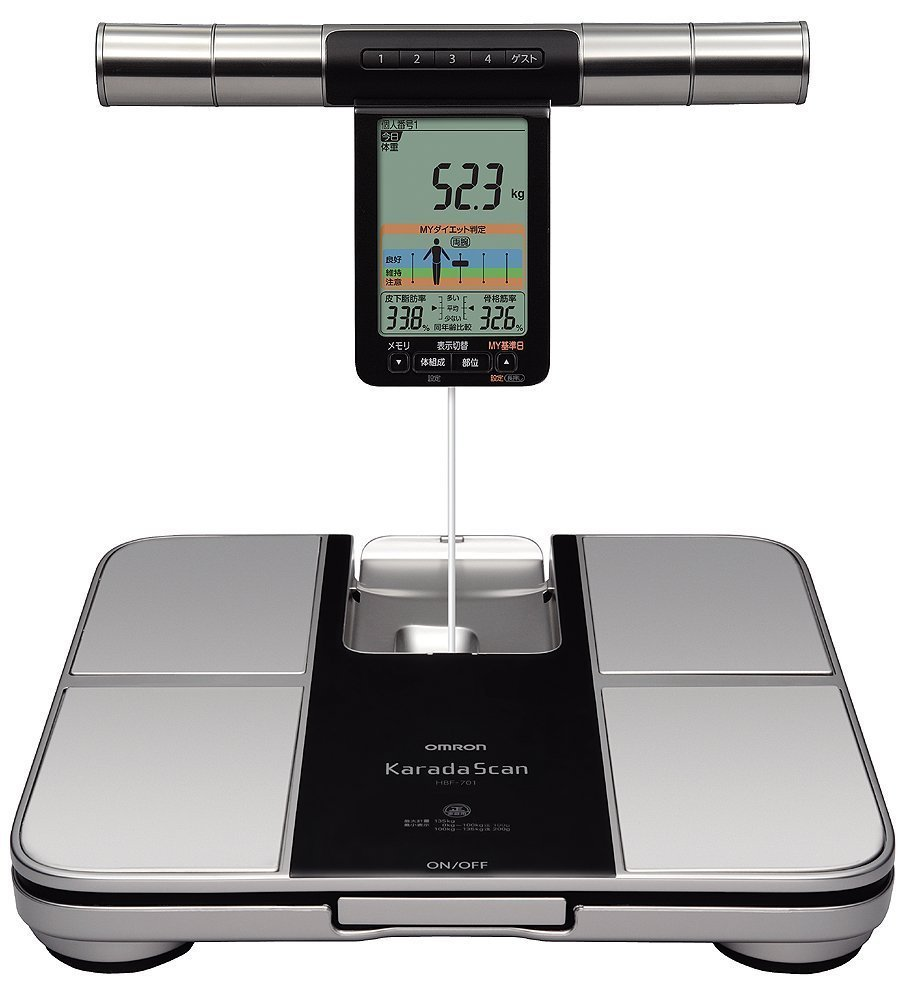
\includegraphics[width=0.8\linewidth]{images/hbf701.jpg}
\end{center}
\section{Getting started}
\label{sec:starting}
The user manual of Omron HBF-516 has useful and valid information for HBF-701
owners. Search for \textit{hbf-516b-instruction-manual.pdf} to download it. For
safety instructions, an introduction to the basic features of the HBF-701, and
operation recommendations read pages 4-13 of
\textit{hbf-516b-instruction-manual.pdf}.

Future versions of this document will include all information needed to operate
the device.

\section{Configuring the HBF-701}
\label{sec:configuring}
Most configurations are done with three keys, arrow up, arrow down and confirm
which is the key that is immediately on the right of arrow down, something like
\begin{CJK}{UTF8}{min}体組成\end{CJK}. The first time you power on the unit, it
may ask for date and time. The first question is about time zone, which is
useless outside Japan.
\begin{enumerate}
  \item For timezone you can select either 1 or 2, using arrow up / down and
	confirm.
  \item Then enter the year, followed by month and day.
  \item Finally enter time in 24 hour format and minutes.
\end{enumerate}

For showing useful results, the HBF-701 need to know your age, sex and height.
It has memory positions for four family members, and an easy way to make
measurements for a guest. The steps below are for configuring the memory
position number 1. Configuring other memory positions, and the guest position is
similar. The guest button is located immediately on the right of the button 4,
and it is something like \begin{CJK}{UTF8}{min}ゲスト\end{CJK}. For configuring
the memory position number 1:
\begin{enumerate}
  \item Power on the unit without lifting the display unit. Wait for it to show
	0.0 kg.
  \item Lift the Display Unit out of the Display Unit Holder, and press the
	button 1.
  \item Enter, using arrows and confirm, your birth date in the following order:
	Year, month, day.
  \item Enter your sex. The male symbol is: \begin{CJK}{UTF8}{min}男\end{CJK}.
  \item Enter your height in centimeters.
  \item If everything went well, then the display will show 0.0 kg, and
	registration is complete.
\end{enumerate}

Now that the device is configured, follow the instructions on pages 25-31 of
\textit{hbf-516b-instruction-manual.pdf} for learning how to take a full or a
weight only measurement. Future versions of this document will include all
information needed to operate the device.

\section{TODO}
\label{sec:todo}
Please help me making this document better by sending pull requests and filling
issues on Github: \url{https://github.com/petersenna/HBF-701}
\begin{itemize}
  \item Make a standalone document without dependency on
	\textit{hbf-516b-instruction-manual.pdf}.
  \item Add pictures.
  \item Include a section on understanding the measurements.
  \item Include a section on how to use the HBF-701 memory function.
\end{itemize}

\section{Legal notice}
\label{sec:legal}
\begin{itemize}
  \item I do not work for Omron. I just own one HBF-701.
  \item I give no warranty about the information on this document. Use the
	information at your own risk.
  \item All trademarks and/or brands cited in this document, including but not
        limited to ``Omron'' are property of their respective owners.
  \item The official manual in Japanese is available at:
        \url{http://www.healthcare.omron.co.jp/product/hbf/hbf-701.html}
  \item This work is licensed under a Creative Commons Attribution 4.0
        International License.
\end{itemize}
\end{document}
